\documentclass[12pt,a4paper]{article}
\usepackage[utf8]{inputenc}
\usepackage{arabtex}
\usepackage{graphicx}
\usepackage{utf8}
\usepackage{hyperref}
\usepackage{subfig}
\usepackage[headheight=0pt,headsep=0pt]{geometry}
\setcode{utf8}
\graphicspath{{Photos/}}
\title{\textbf{Block Filtering}}
\author{Ahmed Osama Mohamed Afifi - 20010038\\\\
Mazen Mohamed Hassanen   - 20011161\\\\
Mohamed Ashraf Elsayed Mahmoud   - 20011488\\\\
Mostafa Mohamed Abdel-Azeem Hassanen  - 20011950\\\\
Ziad Mohamed Mohamed Abdallah Elbouriny - 20010643\\\\}
\date{October 2023}

\begin{document}

\maketitle

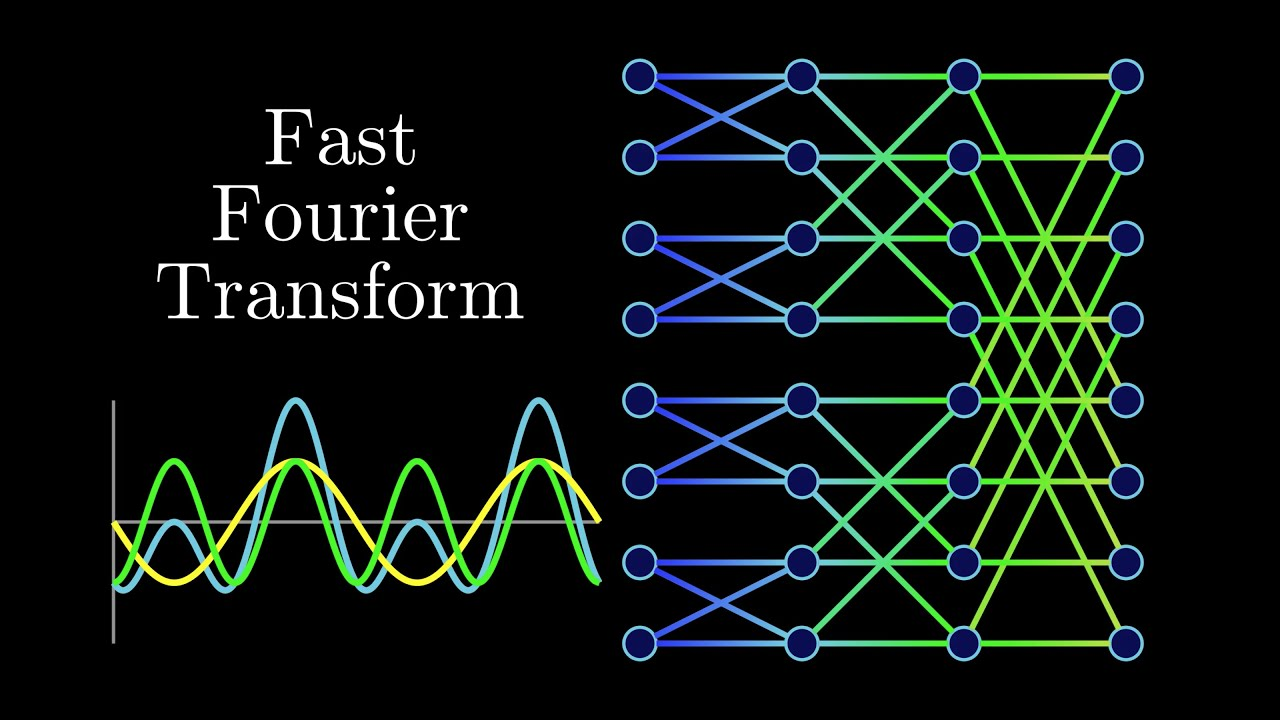
\includegraphics[width=\textwidth]{Photos/maxresdefault.jpg}{\\ \\ \\ \\ \\}
\addtolength{\topmargin}{-60pt}
\addtolength{\textheight}{120pt}
\section*{Introduction}
\large{
There are many DSP applications where a long signal must be filtered in segments. For instance, high-fidelity digital audio requires a data rate of about 5 Mbytes/min, while digital video requires about 500 Mbytes/min. With data rates this high. There are also systems that process segment-by-segment because they operate in real-time. For example, telephone signals cannot be delayed by more than a few hundred milliseconds, limiting the amount of data that is available for processing at any one instant.\\ \\
We must filter the input signal constantly fed into the system to be processed. We want to filter the input blocks as they come
in to be real-time, then we need FFT. There are two methods for segmenting a long input signal into shorter blocks and processing them quickly using the FFT. They are called the Overlap-Add method and the Overlap-Save method.\\

In this report, we will implement both methods using Simulink providing a detailed comparison between both methods.}

\newpage
\section*{Overlap-Save Algorithm}
\large{The overlap-save algorithm filters the input signal in the frequency domain. The input is divided into overlapping blocks which are circularly convolved with the FIR (Finite Impulse Response) filter. For filter length M and FFT size $N$, the first $M-1$ points of the circular convolution are invalid and discarded. The output consists of the remaining $N-M+1$ points, which are equivalent to the true convolution.\\ \\}

\begin{itemize}
\item \textbf {Designing the Filter Kernel}{\\}{\\}
{We will design an FIR filter kernel of length $ M=113$ with frequency specifications, $Fs=8000$, $Fpass=800$ and $Fstop=400$.\\}

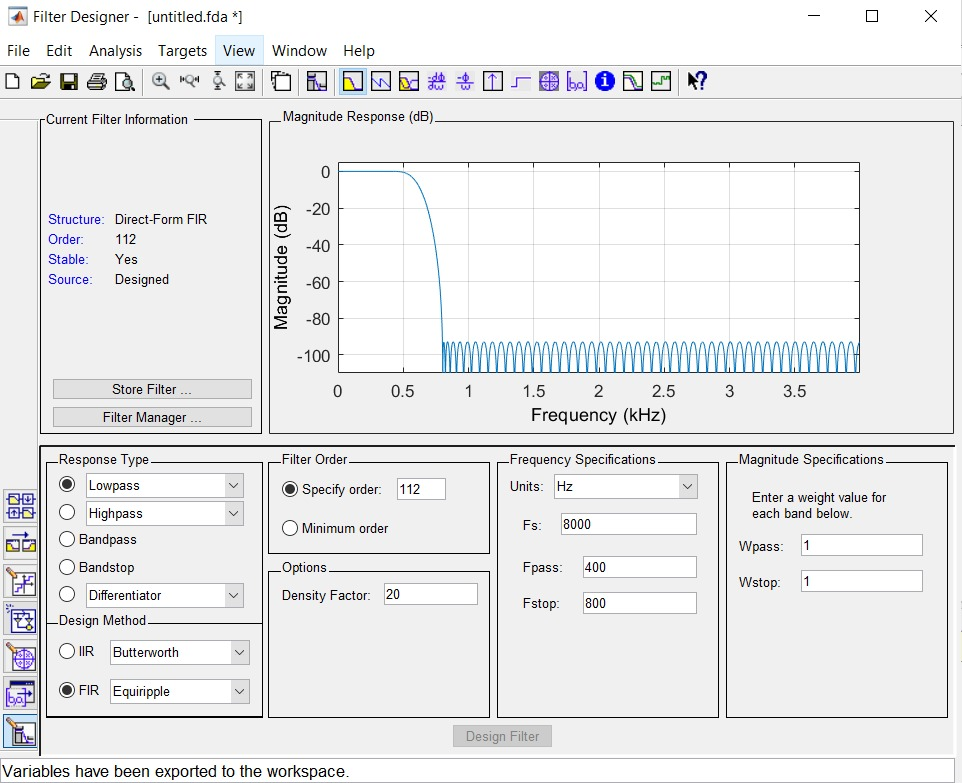
\includegraphics[width=\textwidth]{Photos/overlap save filter.jpeg}
\captionof{figure}{Overlap-Save filter}
\newpage
\item \textbf {Building the Simulink Model}{\\}
{At the very first, we will generate a Sine Wave Source with amplitude $1$ and frequency $100Hz$ and sample time  \(\frac{1}{8000}\). We need to divide the input signal into data block segments of length L, and then we need a buffer, its output is a frame-based signal such that each segment of 400 samples is processed as one chunk, as required by the Overlap-Save process.\\ 
The Overlap-Save algorithm calls for the last M-1 points from the previous data block to be saved and appended to the beginning of the next data block, and then we need to access the previous data block by using a delay which should be set to 400.\\ 
Now, we need to get the M-1 points by adding a Submatrix block to only output the 112x1 column vectors of the 400x1. As explained we need to append the M-1 points to the new block by using a concatenate block. These connections cause the 112×1 vectors from the Submatrix block and the 400×1 vectors from the Buffer (the current data block) to be combined into 512×1 vectors that are suitable for FFT calculation. Our next work is to convolute! By multiplying the FFT computed by the FFT of the filter kernel (FIR).\\ 
Now, we are ready to inverse the FFT to get real output and then the last major step in the Overlap-Save algorithm is to discard all of the points that have aliasing, and then our Overlap-Save Filter is ready!}
\newpage
\item \textbf {Simulink Block Design}{\\}{\\}
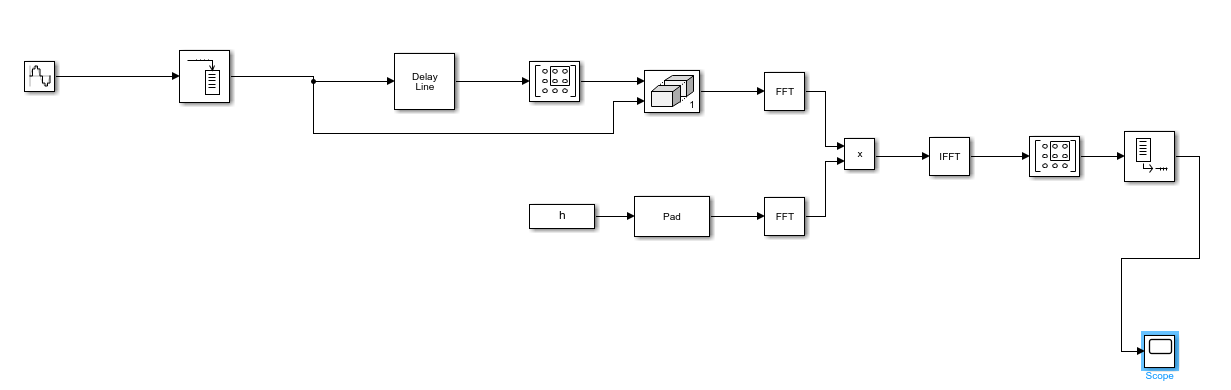
\includegraphics[width=\textwidth]{Photos/overlap save BD.png}
\captionof{figure}{Overlap-Save block diagram}
{Here is the output of Overlap-Save circular convolution. Due to the changes in the FIR there are zero slots in the output.\\ \\}
\newline
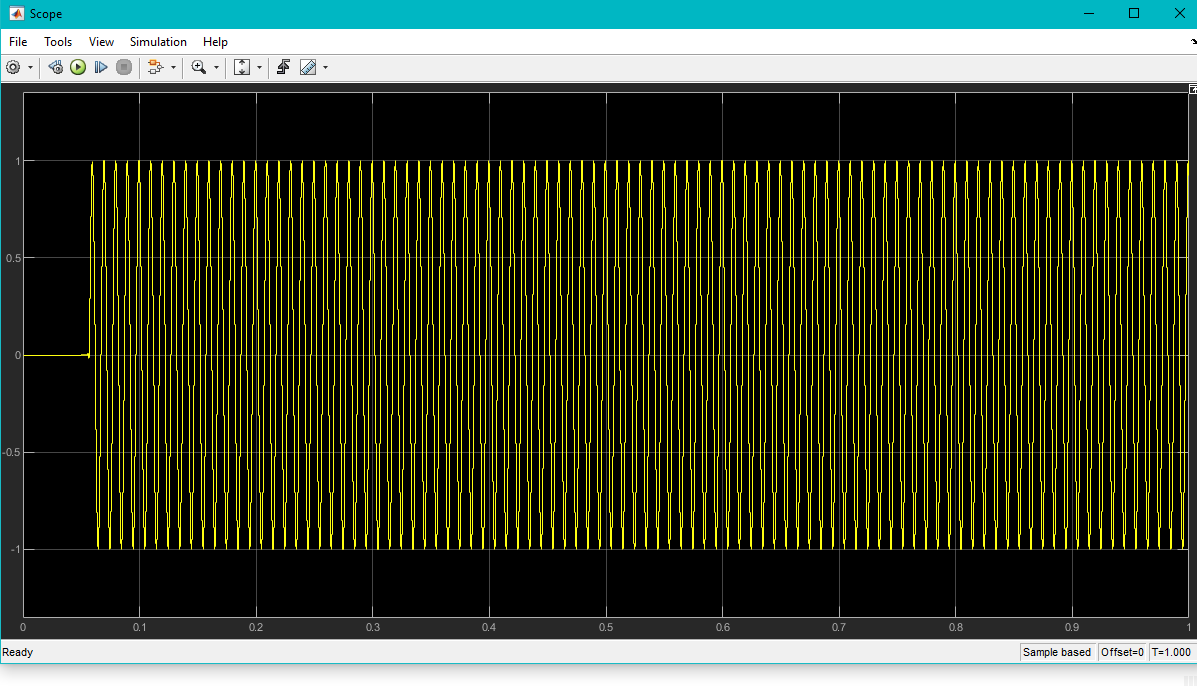
\includegraphics[width=\textwidth]{Photos/overlap save.png}
\captionof{figure}{Overlap-Save output}
\end{itemize}
\newpage
\section*{Overlap-Add Algorithm}

{What is the Overlap-Add method? The Overlap-Add method is based on the fundamental technique in DSP: 
\begin{enumerate}
    \item  decompose the signal into simple components
    \item process each of the components in some useful way
    \item recombine the processed components into the final signal
\end{enumerate}
 The key to this method is how the lengths of these signals are affected by the convolution. When an L sample signal is convolved with an M sample filter kernel, the output signal is $L+M-1$ samples long.\\}
\begin{itemize}
\item \textbf {Designing the Filter Kernel}{\\}{\\}
{Same steps as done for Overlap-Save, but changing its order to 500 such that the length of the filter kernel in M=501. $Fstop$ is changed to $500Hz$.\\ \\}
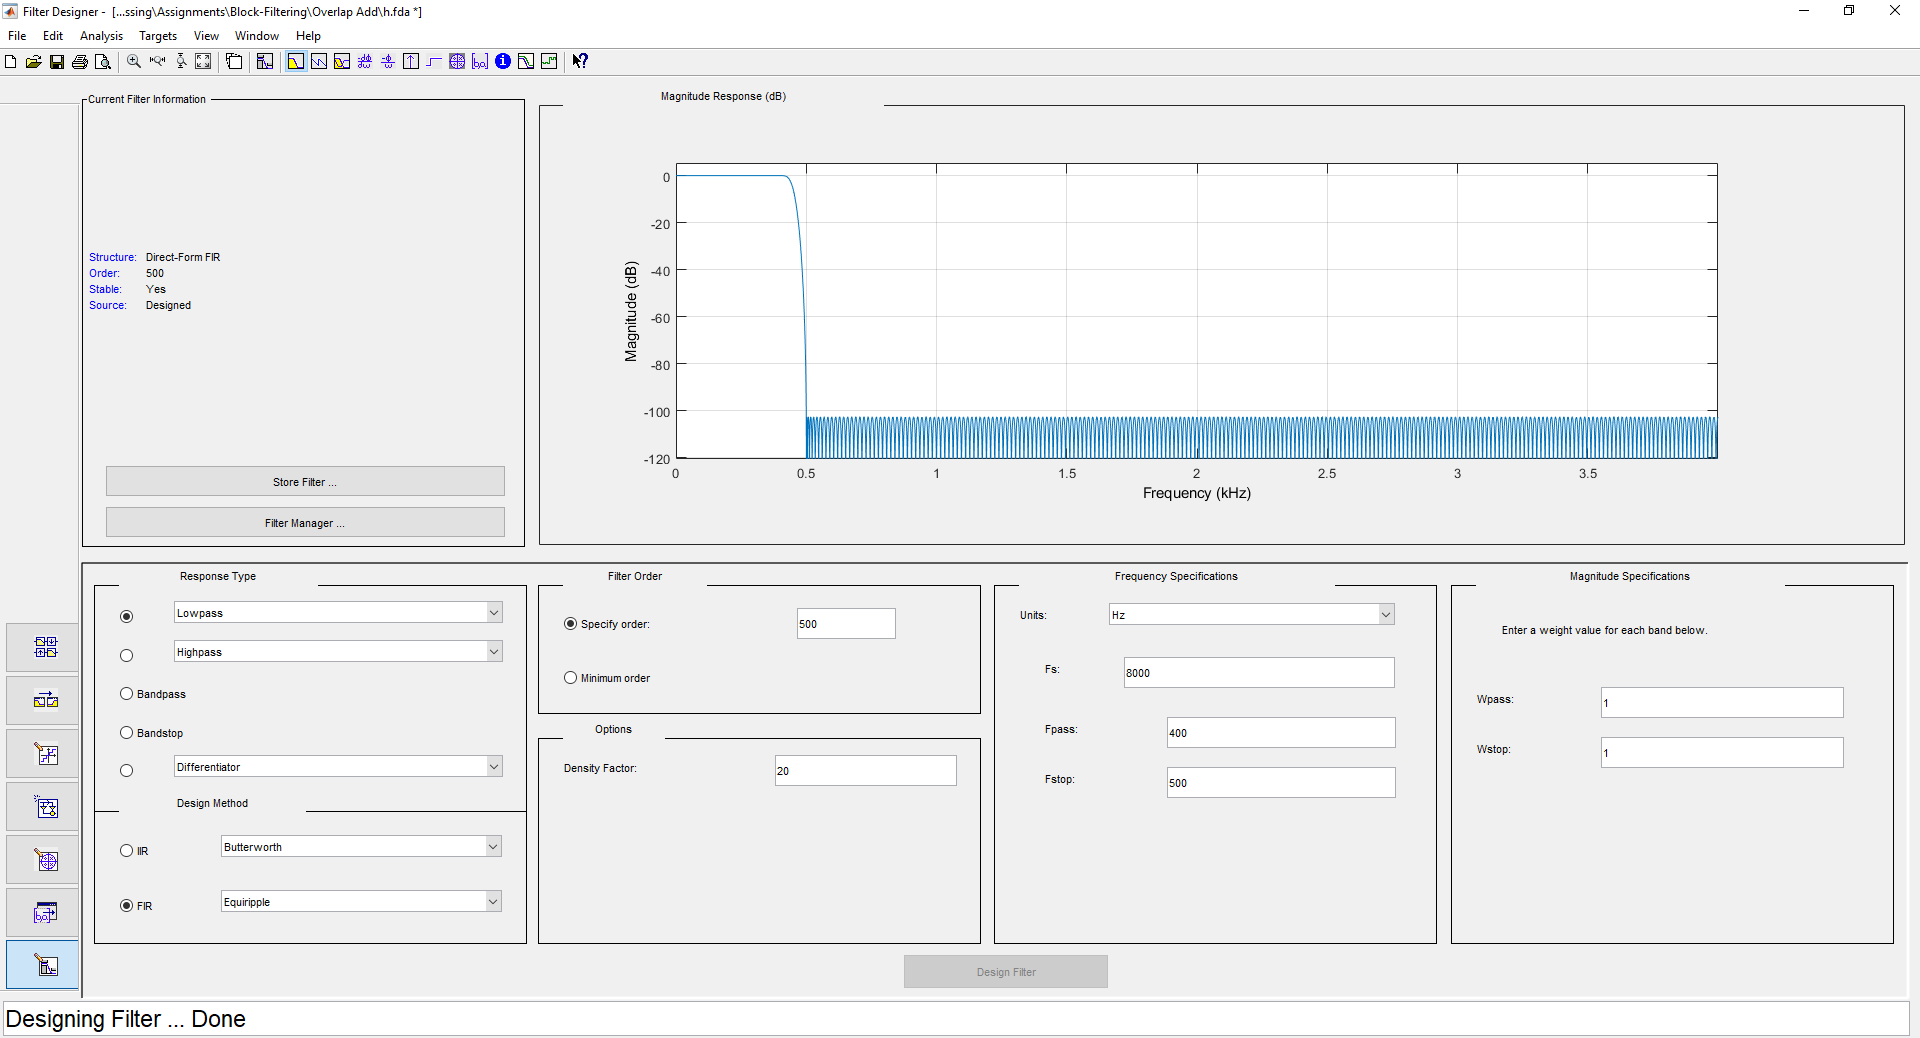
\includegraphics[width=\textwidth]{Photos/overlap add filter.png}
\captionof{figure}{Overlap-Add filter}
\newpage
\item \textbf {Building the Simulink Model}{\\}{\\}
{Dividing the input to the filter into data blocks of $L=1548$, which makes the length of the FFT and IFFT $N=L+M-1=2048$. Now, we will add the same bunch of blocks as done in the Overlap-Save model.}

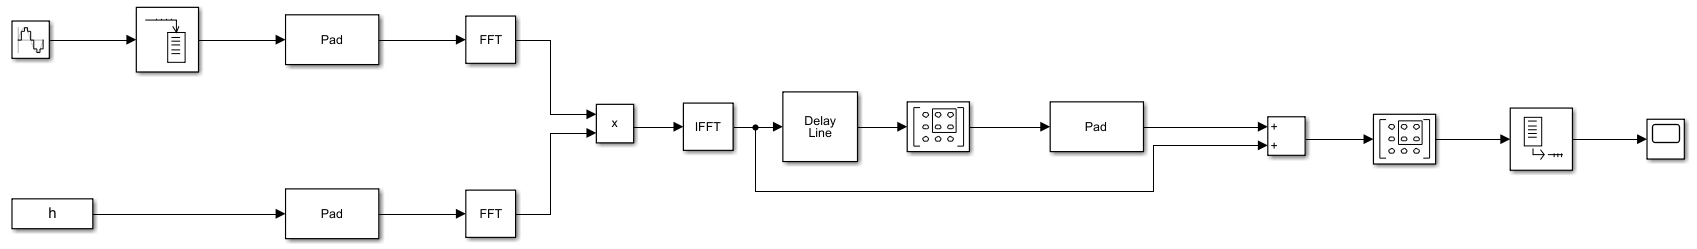
\includegraphics[width=\textwidth]{Photos/overlap add BD.png}
\captionof{figure}{Overlap-Add block diagram}

{Here is the output of Overlap-Add circular convolution. Due to the changes in the FIR there are zero slots in the output.\\ \\}
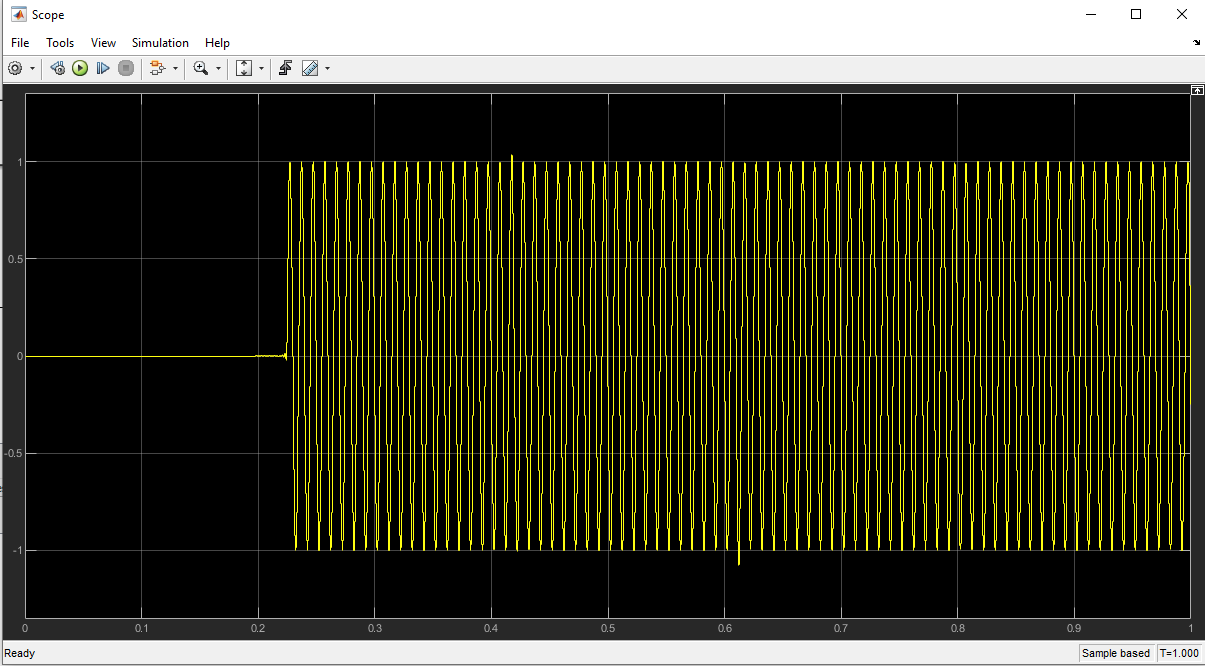
\includegraphics[width=\textwidth]{Photos/overlap add.png}
\captionof{figure}{Overlap-Add output}

\end{itemize}
\newpage
\section*{Linear Convolution}


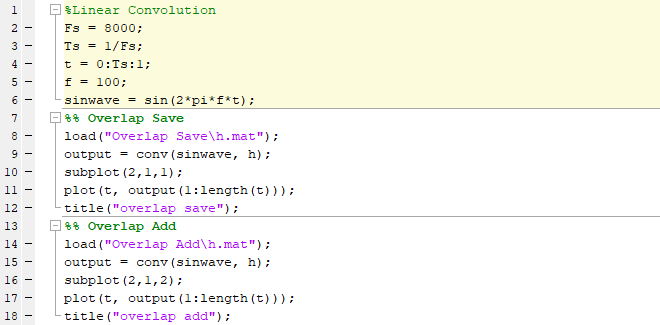
\includegraphics[width=\textwidth]{Photos/linear convolution code.png}
\captionof{figure}{Linear convolution code}
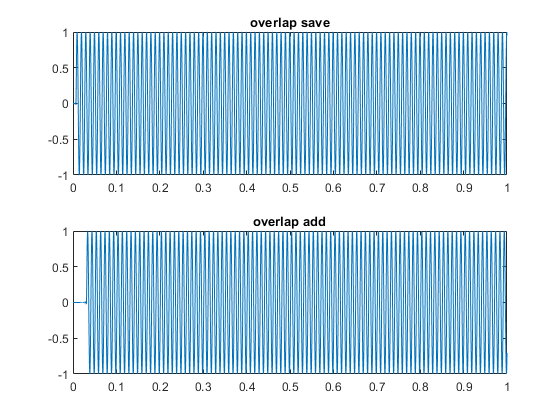
\includegraphics[width=\textwidth]{Photos/linear convolution.png}
\captionof{figure}{Linear convolution output}

\end{itemize}
\newpage
\section*{Overlap-Save Vs Overlap-Add}
{Here is a simple summary of differences between overlap add and overlap save that might influence which one you use:}
\begin{itemize}

\item{Overlap add will involve adding a number of values in the output to recover the final signal, whereas overlap save does not require any addition in this step.  This might be important to you if you want to consider the numerical precision of your output, or if you want to reduce the number of addition operations.}
\item{The Overlap add method can be computed using linear convolution since the zero padding makes the circular convolution equal to linear convolution in these cases.}
\item{The Overlap save method doesn't do as much zero padding but instead re-uses values from the previous input interval.  In overlap save, some values are considered contaminated due to the aliasing of the circular convolution, so they are discarded from the output.}
\item{In overlap save there is less zero padding.  In fact, the only time you need to zero pad is before the first interval, and after the last interval if the length of the input sequence isn't evenly divided by L.}
\end{itemize}

\end{document}
